\documentclass{beamer}

\mode<presentation> {
\usetheme{CambridgeUS}
\usecolortheme{dalhousie}
}

\usepackage{graphicx} % Allows including images
\usepackage{booktabs} % Allows the use of \toprule, \midrule and \bottomrule in tables
\usepackage{tikz}
%\usepackage[outdir=./]{epstopdf}
\setbeamerfont{section number projected}{%
	family=\rmfamily,series=\bfseries,size=\normalsize}
\setbeamercolor{section number projected}{bg=black,fg=dalgold}

\setbeamerfont{subsection number projected}{%
	family=\rmfamily,series=\bfseries,size=\normalsize}
\setbeamercolor{subsection number projected}{bg=dalblack!70,fg=dalgold}

%----------------------------------------------------------------------------------------
%	TITLE PAGE
%----------------------------------------------------------------------------------------

\title[AMID]{Atlung Method for Intercalant Diffusion --- AMID}

\author{Marc M. E. Cormier} % Your name
\institute[] % Your institution as it will appear on the bottom of every slide, may be shorthand to save space
{
	Dalhousie University \\ % Your institution for the title page
	\medskip
	\textit{marc.cormier@dal.ca} % Your email address
}
\date{June 21, 2021} % Date, can be changed to a custom date

\begin{document}
	
\begin{frame}
\titlepage % Print the title page as the first slide
\end{frame}

\begin{frame}
\frametitle{Theory of Diffusion}

	\begin{equation*}
	\vec{j} = -D \vec{\nabla}(c);\ \frac{\partial c}{\partial t} = D \nabla^2(c)
	\end{equation*}
	\begin{itemize}
		\item A continuum theory: $\nabla$ is derivative w.r.t. to spatial coordinates.
		\item $c$ is the Li concentration and depends on the spatial coordinate of the particle and time: $c(x,y,z,t)$ or $c(\theta,\phi,r,t)$
		\item For \emph{spheres}, $c$ is assumed to be spherically symmetric $\rightarrow$ only depends on $r$.
		\item {\color{red} Assumes D is \emph{not} concentration dependent ... !}
		\item These are coupled partial differential equations. Generally very difficult to solve.
	\end{itemize}
	 
\end{frame}

\begin{frame}
\frametitle{General Solution}

\begin{equation*}
c(t,x) = \frac{j_0 r}{D} \left[ a\frac{Dt}{r^2} + \frac{z^2}{2} - b - 2 \sum_{i} \frac{\exp(-\alpha_i^2Dt/r^2)}{\alpha_i^2} C(\alpha_i z) \right]
\end{equation*}

Where $z=x/r$ is a normalized coordinate \\ 
$\rightarrow z=1$: surface, $z=0$: center.

\begin{figure}
	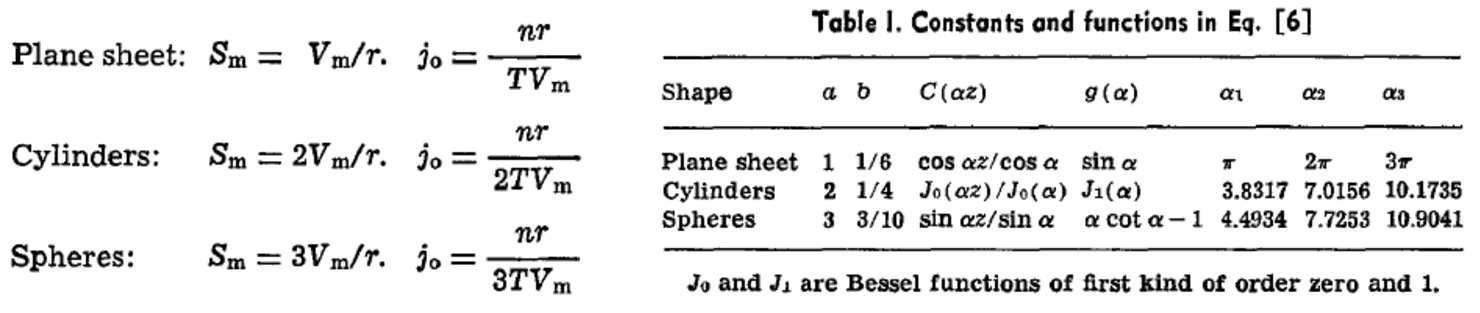
\includegraphics[width=1.0\linewidth]{figs/diff_eqn_parameters.pdf}
\end{figure}

$j_0$ is a flux density that depends on the particle shape. This assumes that on average, all areas of particle surfaces see the same amount of Li ions enter the material (all surfaces are equally active).


\end{frame}

\begin{frame}
\frametitle{Normalized Solution (for spheres)}

\begin{equation*}
X(z, \tau) = \tau + \frac{1}{3Q} \left(\frac{z^2}{2} - \frac{3}{10} -2 \sum_{i} \left[\frac{\exp(-\alpha_i^2 Q\tau)}{\alpha_i^2} \frac{\sin(\alpha_i z)}{\sin(\alpha_i)} \right] \right)
\end{equation*}
\begin{itemize}
	\item $X = \frac{cV_m}{n}$: local fractional Li concentration.
	\item $z = x/r$: normalized coordinate  $\rightarrow z=1$: surface, $z=0$: center.
	\item $\tau = t/T$; \\
		  $T$: capacity/current ((dis)charge time), $t$: elapsed (dis)charge time\\ 
		  $\therefore \tau=$ fractional capacity
	\item $Q = T/(r^2/D)$; \\
		  $(r^2/D)$ is characteristic diffusion time (average time it takes a Li ion to travel from center to surface) \\
		  $\therefore Q$ is fractional time: ((dis)charge time) / (diffusion time)
\end{itemize}

\end{frame}

\begin{frame}
\frametitle{Solution, at the surface}

At the surface, $x=r \therefore z=1$, and denote $X(z=1, \tau) = X^*(\tau)$:
\begin{equation*}
X^*(\tau) = \tau + \frac{1}{AQ} \left[ \frac{1}{B} - 2 \sum_{i}\frac{\exp(-\alpha_i^2 Q\tau)}{\alpha_i^2}  \right]
\end{equation*}
Where, 
\begin{figure}
	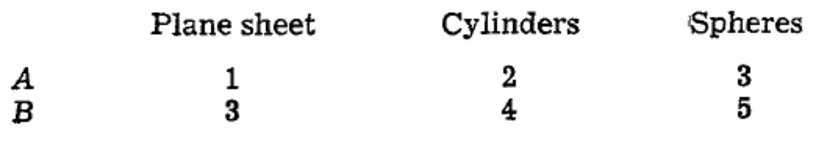
\includegraphics[width=0.65\linewidth]{figs/atlung_constants.pdf}
\end{figure}

\end{frame}

\begin{frame}
\frametitle{What about the $\alpha_i$'s?}

From Table 1, the generating functions are:

\begin{itemize}
	\item Plane sheet: $g(\alpha) = \sin(\alpha)$
	\item Cylinders: $g(\alpha) = J_1(\alpha)$
	\item Spheres: $g(\alpha) = \alpha \cot(\alpha) - 1$
\end{itemize}

$\alpha_i$ are the roots of the generaing equations $\rightarrow g(\alpha_i) = 0$

There are infinitely many solutions for each shape! For spheres, 
\begin{equation*}
\alpha_i \cot(\alpha_i) = 1
\end{equation*}
 
\end{frame}

\begin{frame}
\frametitle{Everyone has seen, but where does it come from?}

\vspace{-0.45cm}
\begin{figure}
	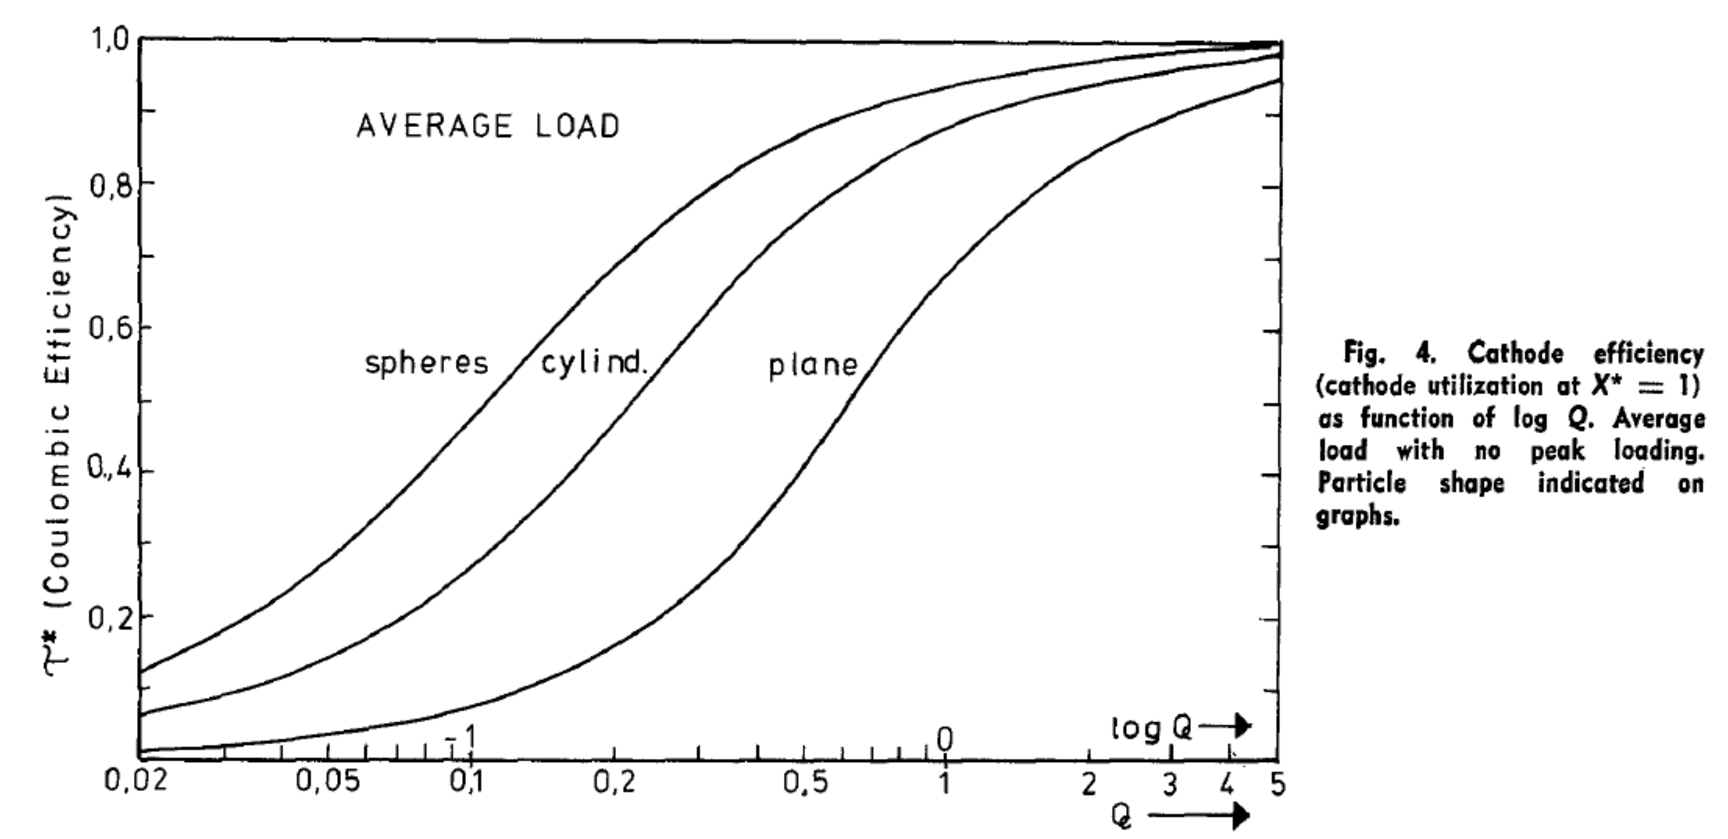
\includegraphics[width=0.75\linewidth]{figs/tau_vs_Q-original.pdf}
\end{figure}

\vspace{-0.1cm}
$\tau^*$ is the fractional capacity when $X^*=1$ (i.e., when the surface concentration reaches its (fractional) saturation value):
\begin{equation*}
X^* = 1 = \tau^* + \frac{1}{AQ} \left[ \frac{1}{B} - 2 \sum_{i}\frac{\exp(-\alpha_i^2 Q\tau^*)}{\alpha_i^2}  \right]
\end{equation*}

\end{frame}

\begin{frame}
\frametitle{Everyone has seen, but where does it come from? (cont'd)}

\begin{equation*}
\tau^* + \frac{1}{AQ} \left[ \frac{1}{B} - 2 \sum_{i}\frac{\exp(-\alpha_i^2 Q\tau^*)}{\alpha_i^2}  \right] = 1
\end{equation*}

is an \emph{implicit} equation of $\tau^*$ and $Q$. There is no analytical solution, must be solved numerically to get: \\
\begin{equation*}
\tau^*(Q)
\end{equation*}

The result is sensitive to the number of $\alpha_i$'s inlcuded in the expansion...

\end{frame}

\begin{frame}
\frametitle{Numerical solutions for spheres}

\begin{figure}
	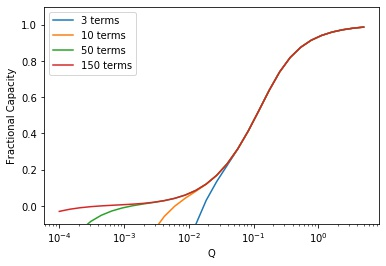
\includegraphics[width=0.65\linewidth]{figs/Atlung_spheres_alpha_expansion.jpg}
\end{figure}

\end{frame}

\begin{frame}
\frametitle{How do we get D?}

Recall that $Q=T/(r^2/D)$. But since $T$ is the (dis)charge time, $T=3600n$, for $n$ in $C/n$. 
\begin{equation*}
\therefore Q = \frac{3600nD}{r^2}
\end{equation*} 

\begin{equation*}
\therefore \tau^* + \frac{r^2}{3600nDA} \left[ \frac{1}{B} - 2 \sum_{i}\frac{\exp(-3600nD\alpha_i^2 \tau^*/r^2)}{\alpha_i^2}  \right] = 1
\end{equation*}

If the particle size, $r$, is known, then this equation relates the fractional capacity, $\tau^*$ to the rate, $n$, for a given $D$.

$\Rightarrow$ Capacity-rate data can be fit to this expression to extract $D$! \\
(We actually write $\tau=c/c_{max}$, where $c_{max}$ is maximum available capacity, in case the lowest rate did not achieve saturation capacity)

\end{frame}

\begin{frame}
\frametitle{Capacity-rate data}

\begin{center} 
	Li$_{1.12}$Ni$_{0.44}$Mn$_{0.44}$O$_2$
\end{center}
\vspace{-0.5cm}
\begin{figure}
	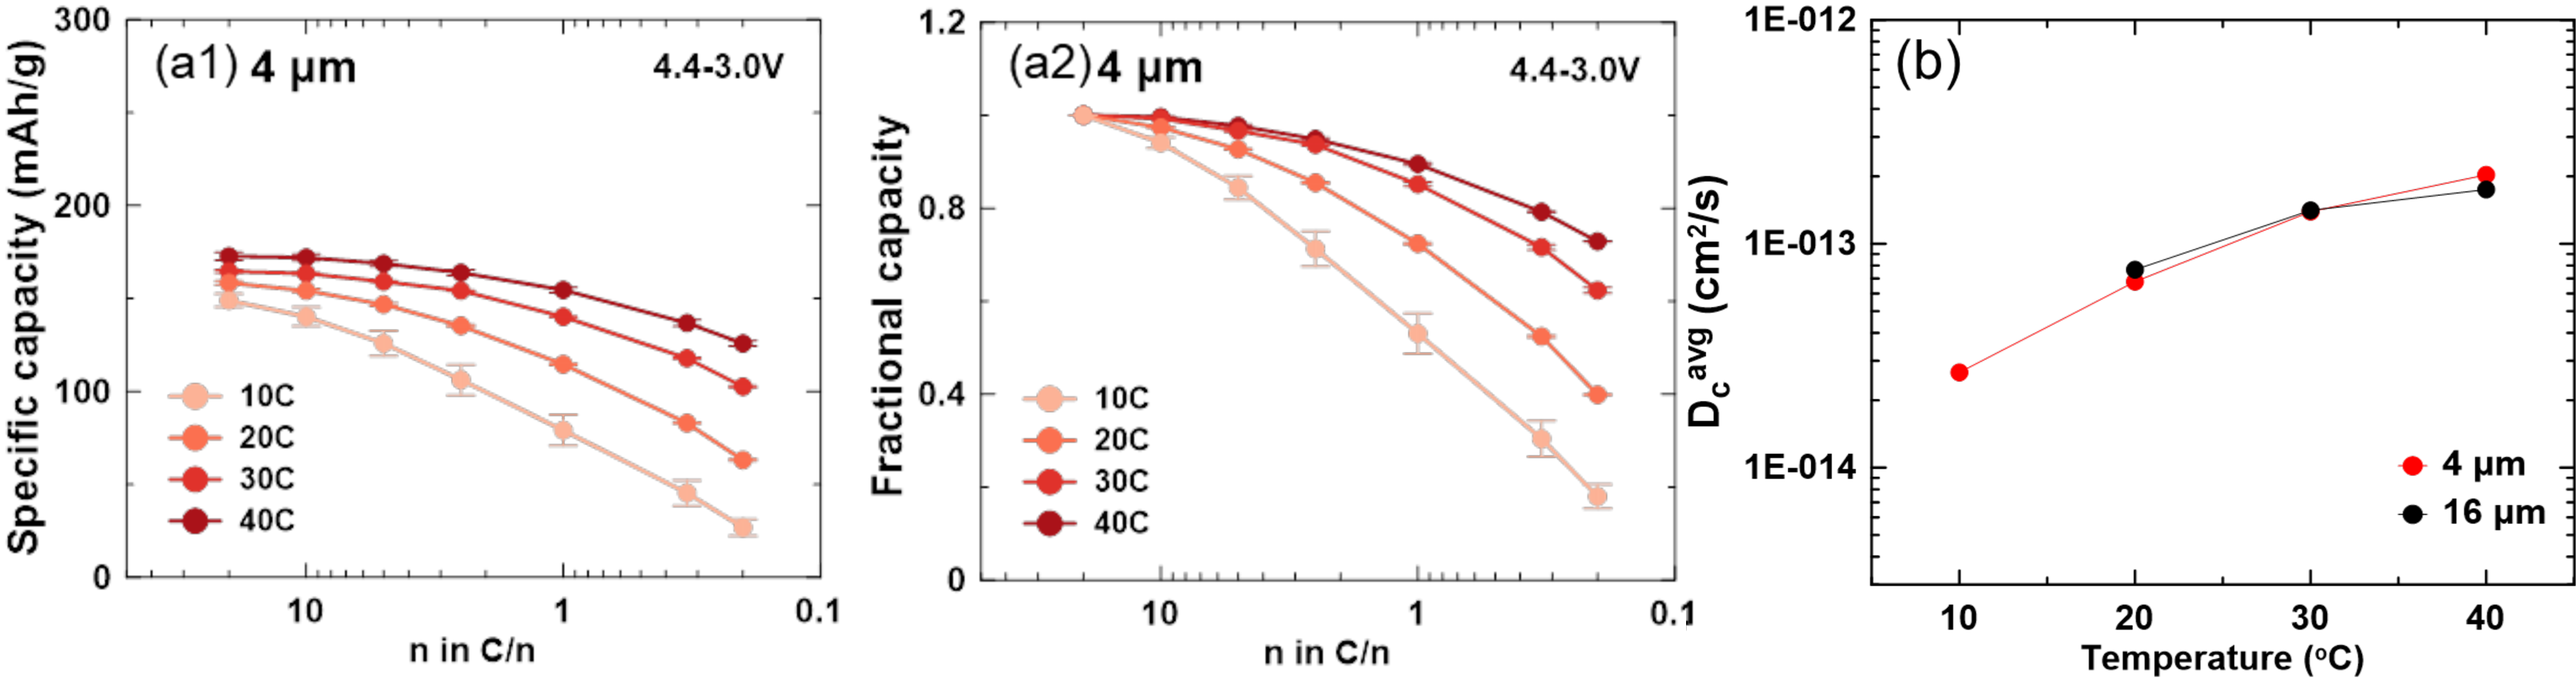
\includegraphics[width=0.9\linewidth]{figs/cap-rate_D-T.pdf}
\end{figure}

In this case, we can extract $D$ as a function of $T$ (temperature); each curve can be fit to the equation on the previous slide. \\
There is a problem here: recall that $D$ is supposed to be constant - but it is NOT constant in the $4.4-3.0$ V interval! \\
\vspace{\baselineskip}
\footnotesize K.K. paper, N.P.

\end{frame}

\begin{frame}
\frametitle{Getting capacity-rate data: signature curves}

\begin{figure}
	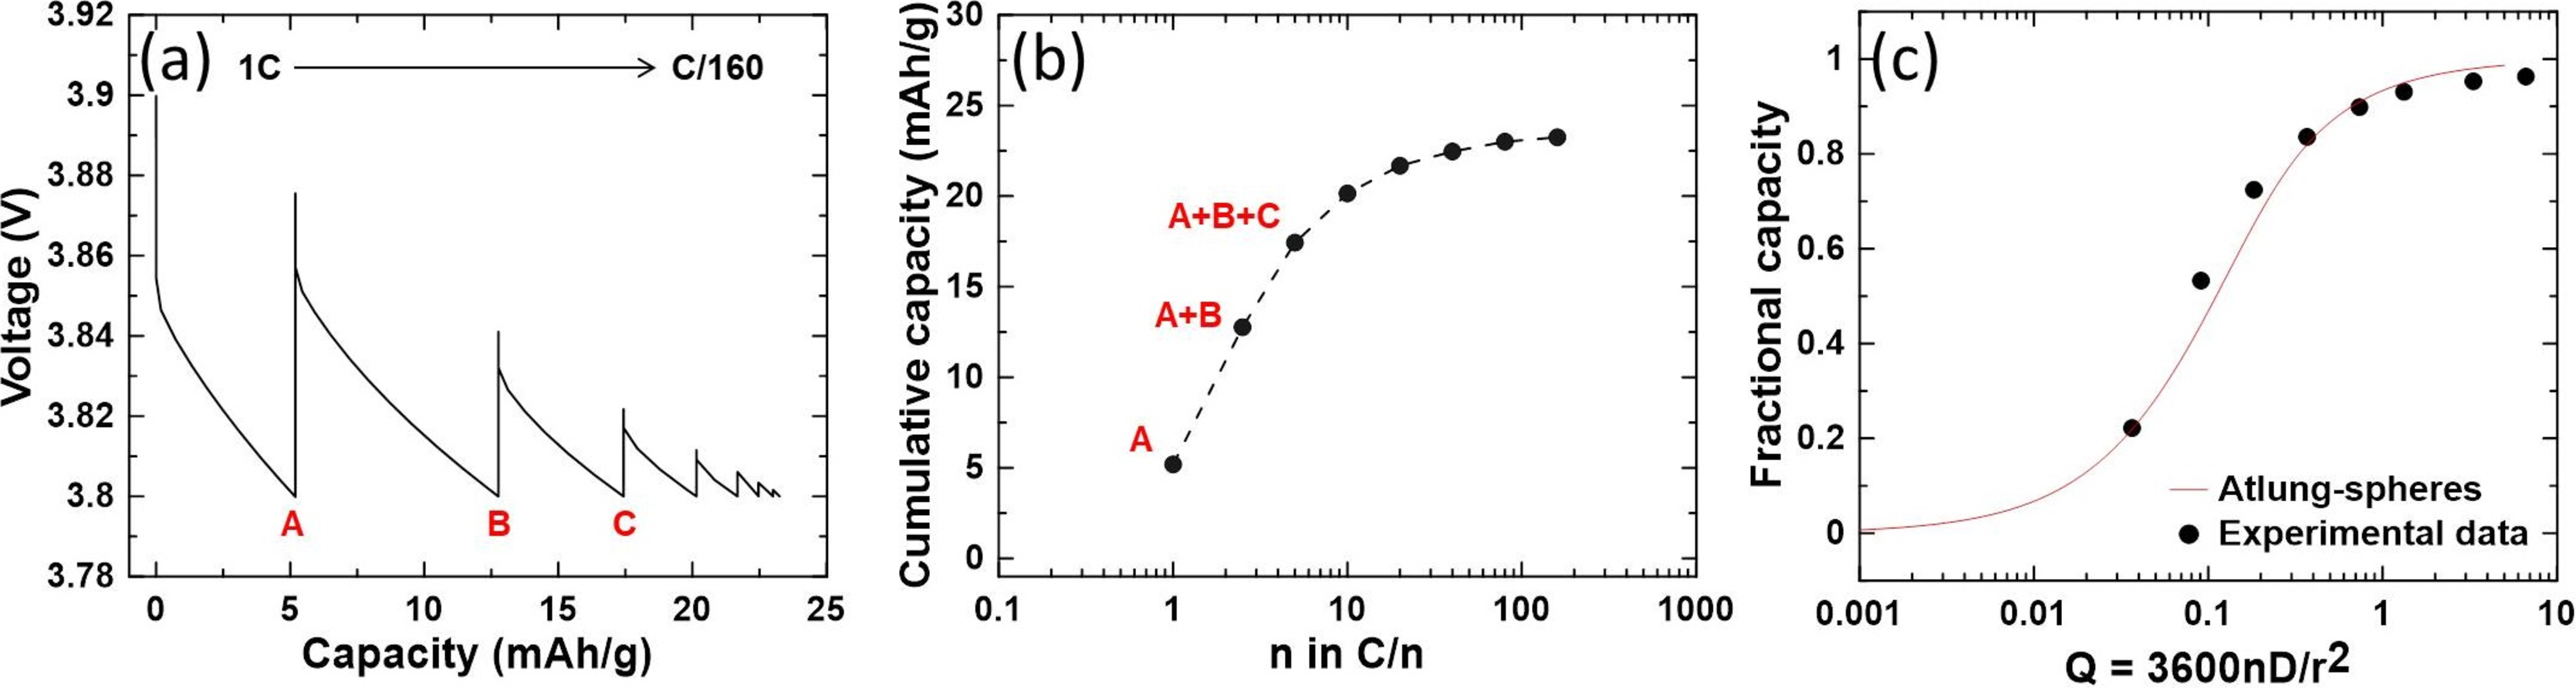
\includegraphics[width=0.85\linewidth]{figs/sig_curves.pdf}
\end{figure}
\vspace{-0.5cm}
Signature curve: sequential (dis)charge at lower and lower rates with OCV in between. 
\begin{itemize}
	\item Fix voltage interval
	\item Fix OCV time.
	\item Select rates.
\end{itemize}
Should give the same cumulative capacity for each rate. Much faster than charging back to starting V each time and does not require CV holds. \\
\vspace{\baselineskip}
\footnotesize KH paper, A.L., N.P.

\end{frame}

\begin{frame}
\frametitle{D(V): advanced signature curve protocol}

\centering Li$_{1.12}$Ni$_{0.44}$Mn$_{0.44}$O$_2$
\vspace{-0.25cm}
\begin{figure}
	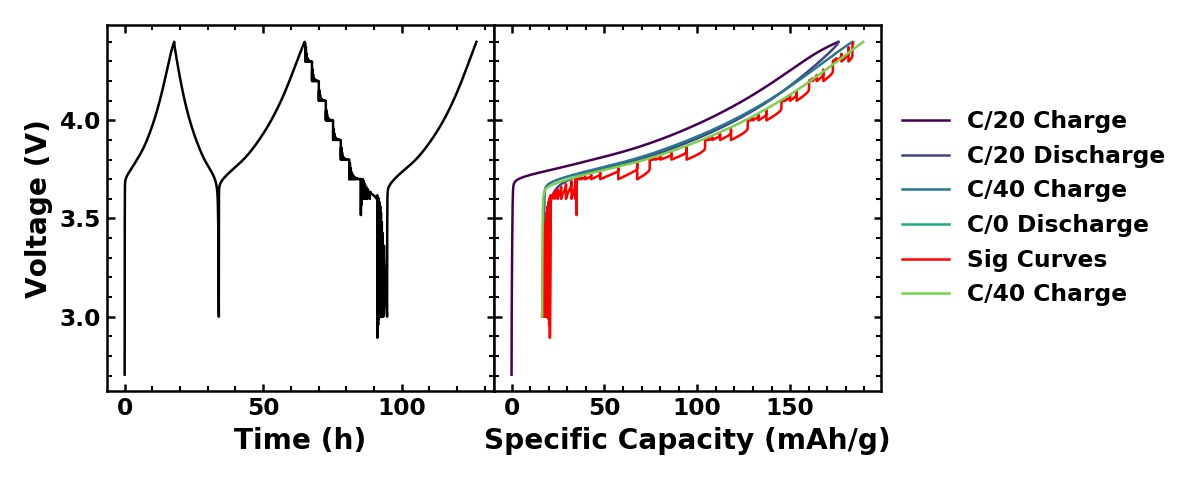
\includegraphics[width=0.85\linewidth]{figs/protocol_vis_Li112Ni44Mn44O2.jpg}
\end{figure}
\vspace{-0.5cm}
\begin{itemize}
	\item This protocol performs sequential signature curves within $0.1$ V intervals from $4.4-3.6$ V and one $0.6$ V interval from $3.6-3.0$ V
	\item Note the C/0 discharge --- this is an OCV at top of charge before signature curves begin and \emph{should not} be there.
\end{itemize}

\end{frame}

\begin{frame}
\frametitle{D(V): capacity-rate data and effective rates}

\begin{columns}
	\column{0.55\textwidth}
	\centering Li$_{1.12}$Ni$_{0.44}$Mn$_{0.44}$O$_2$
	\vspace{-0.3cm}
	\begin{figure}
		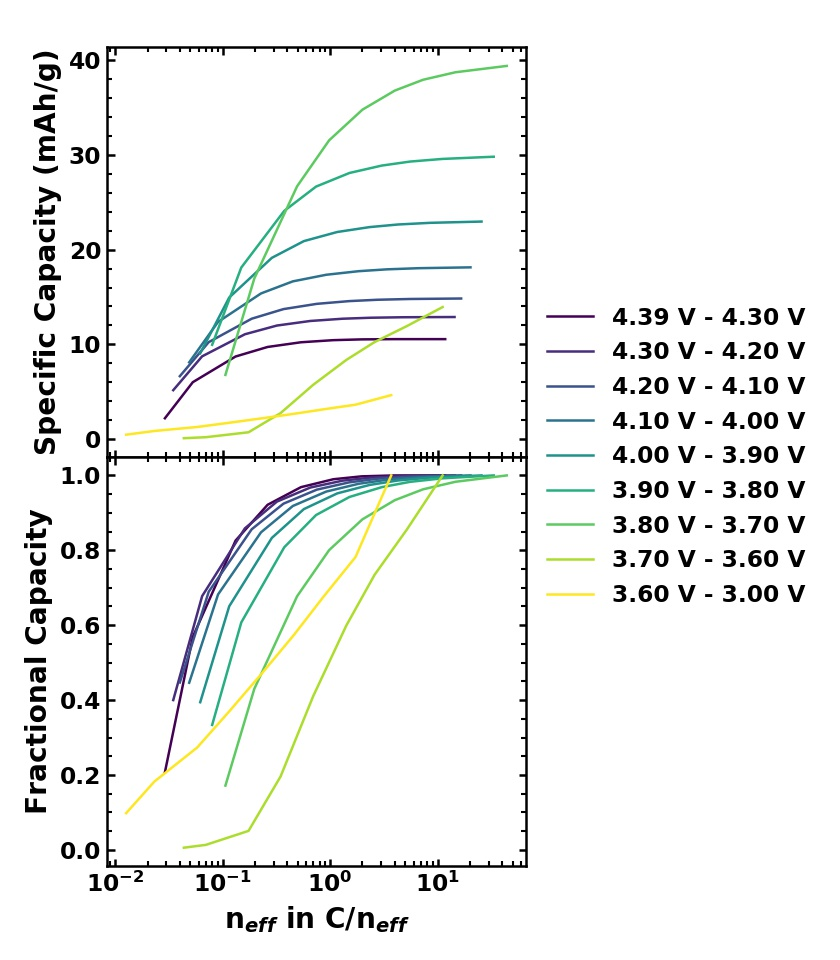
\includegraphics[width=0.95\linewidth]{figs/cap-rate_Li112Ni50Mn50.jpg}
	\end{figure}

	\column{0.45\textwidth}
	What is the (dis)charge time for an arbitrary voltage interval? \\
	\vspace{\baselineskip}
	Since the capacity within each votlage interval is not known \emph{a priori}, currents input in the protocal are determined from the full theoretical capacity.\\
	\vspace{\baselineskip}
	The (dis)charge time, $3600n$, to be used in the fit must be computed for each voltage interval based on the cumulative capacity achieved within that interval.

\end{columns}

\end{frame}


\begin{frame}
\frametitle{D(V): IR contribution to V}

\begin{figure}
	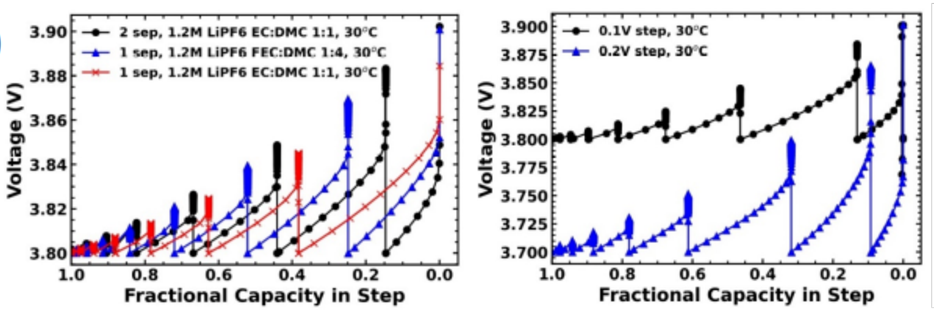
\includegraphics[width=0.95\linewidth]{figs/IR_eg.pdf}
\end{figure}
\vspace{-0.5cm}
\begin{itemize}
	\item Coin cells for diffusion measurement must be constructed to minimize IR contributions to V.
	\item Larger V intervals can help, but remember that $D$ is supposed to be constant. 
\end{itemize}

\footnotesize AMID: How-to, EZ

\end{frame}


\begin{frame}
\frametitle{D(V): fits}

\begin{columns}
	
	\column{0.5\textwidth}
	\centering A bad fit
	\vspace{-0.4cm}
	\begin{figure}
		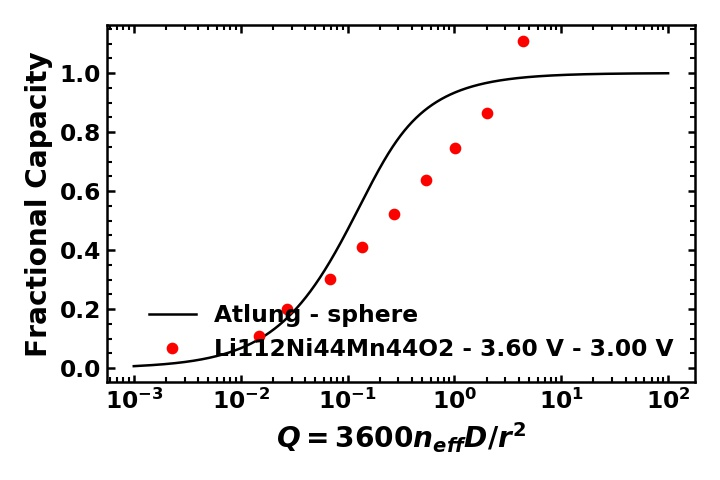
\includegraphics[width=0.95\linewidth]{figs/Li112Ni44Mn44O2_Atlung-sphere_3300.jpg}
	\end{figure}
	
	\column{0.5\textwidth}
	\centering A good fit
	\vspace{-0.4cm}
	\begin{figure}
	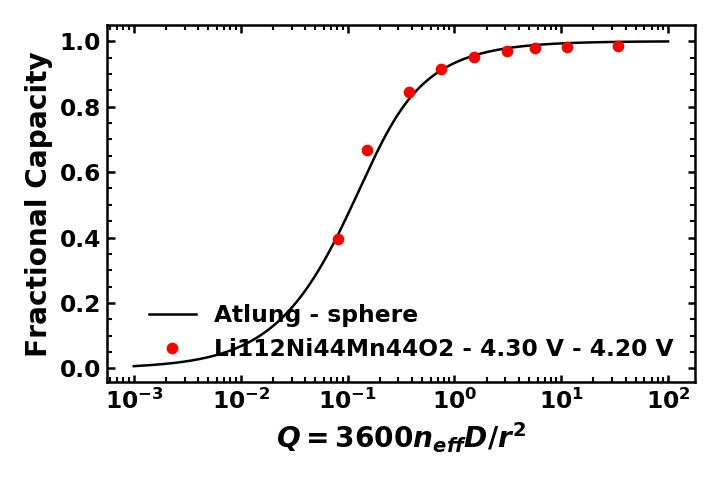
\includegraphics[width=0.95\linewidth]{figs/Li112Ni44Mn44O2_Atlung-sphere_4250.jpg}
	\end{figure}
	
\end{columns}

Once $D$ and $c_{max}$ are fit, we can plot the measured data on top of the theoretical $\tau^*(Q)$ curve to get a visual of fit quality. \\
\vspace{\baselineskip}
The weight of each rate in the fit is scaled by the magnitude of the IR contribution to V. 

\end{frame}

\begin{frame}
\frametitle{D(V): fit quality}

\begin{columns}
	\fontsize{10}{8}
	
	\column{0.45\textwidth}
	\vspace{-0.5cm}
	\begin{figure}
		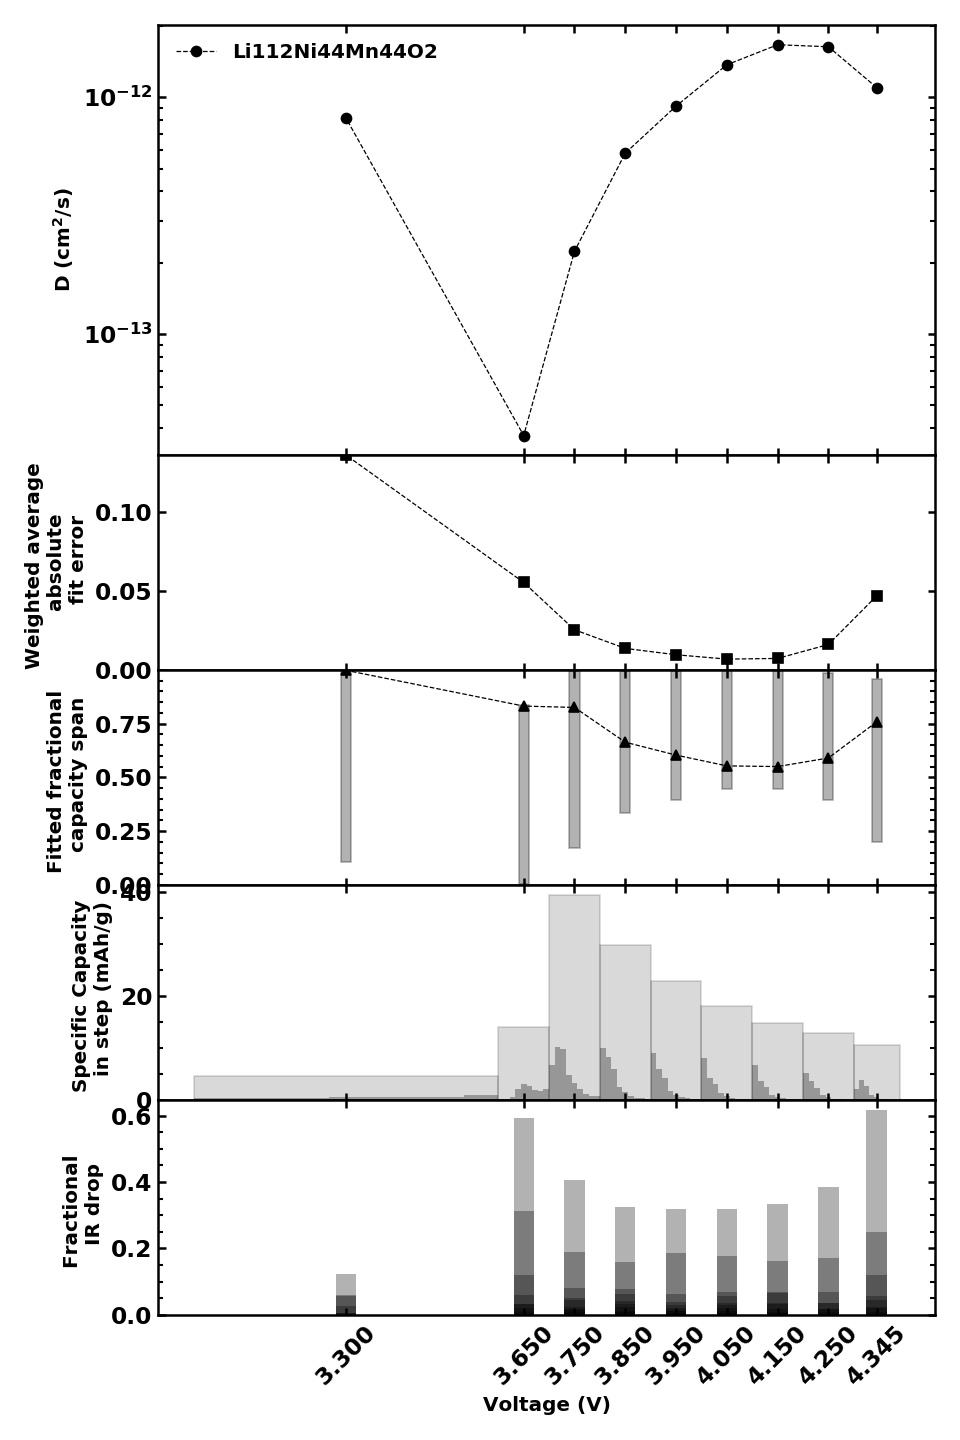
\includegraphics[width=0.95\linewidth]{figs/D-V_Li112Ni44Mn44O2_r-05um.jpg}
	\end{figure}
	
	\column{0.55\textwidth}
	\begin{itemize}
		\item Average fit error $= \sum_{i=1}^{n_{rates}}IR^{norm}_{i}|\tau_i - \tau_{Atlung}|$ 
		\item Capacity span: which portion of the theoritical curve is covered by the fitted data.\\
			  Length of grey bar $\rightarrow$ black triangle
		\item Specific capacities: light grey bars give cumulative capacity achieved in each voltage interval; 
		      dark grey bars gives additional capacity achieved at each rate. The sum of the dark grey bars give the height of their respective light grey bar.
		\item IR drop: Sequentially darker shades correspond to sequentially lower rates. Lightest shade $\rightarrow$ highest rate. Computed by 
			  dividing IR for a particular rate by the size of the voltage interval. 
	\end{itemize}
	
\end{columns}

\end{frame}

\begin{frame}
\frametitle{Particle size}

\begin{figure}
	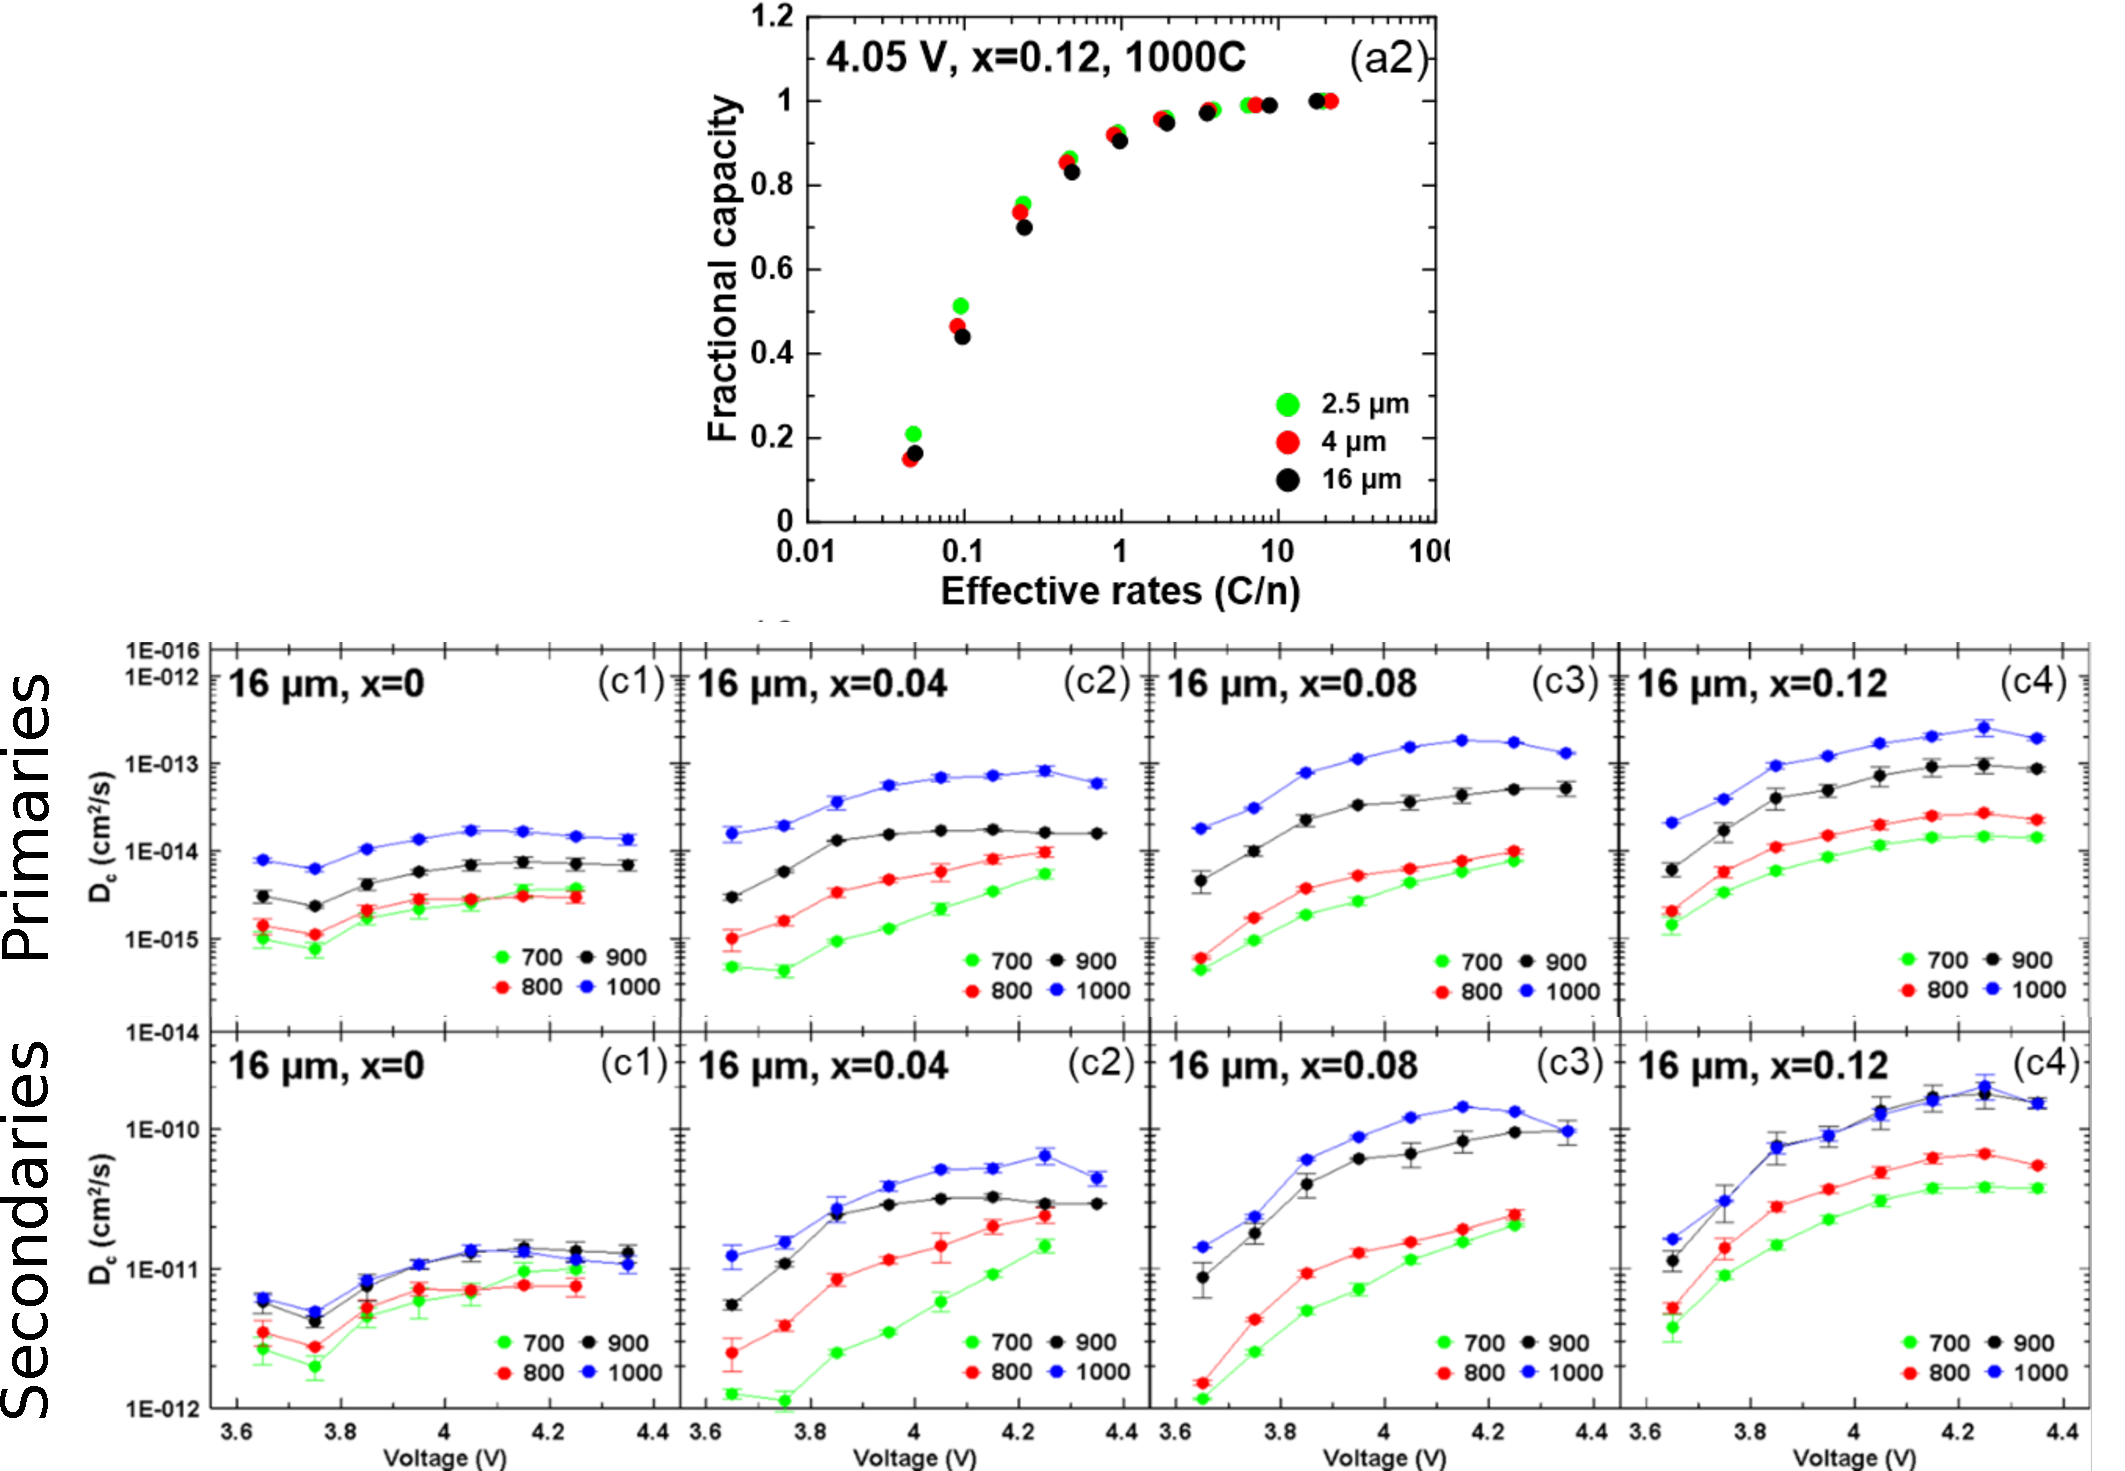
\includegraphics[width=0.85\linewidth]{figs/prim_vs_sec_particles.pdf}
\end{figure}

\end{frame}

\begin{frame}
\frametitle{Particle shape}

\centering
SC-LiNi$_{0.975}$Mg$_{0.025}$O$_2$
\begin{figure}
	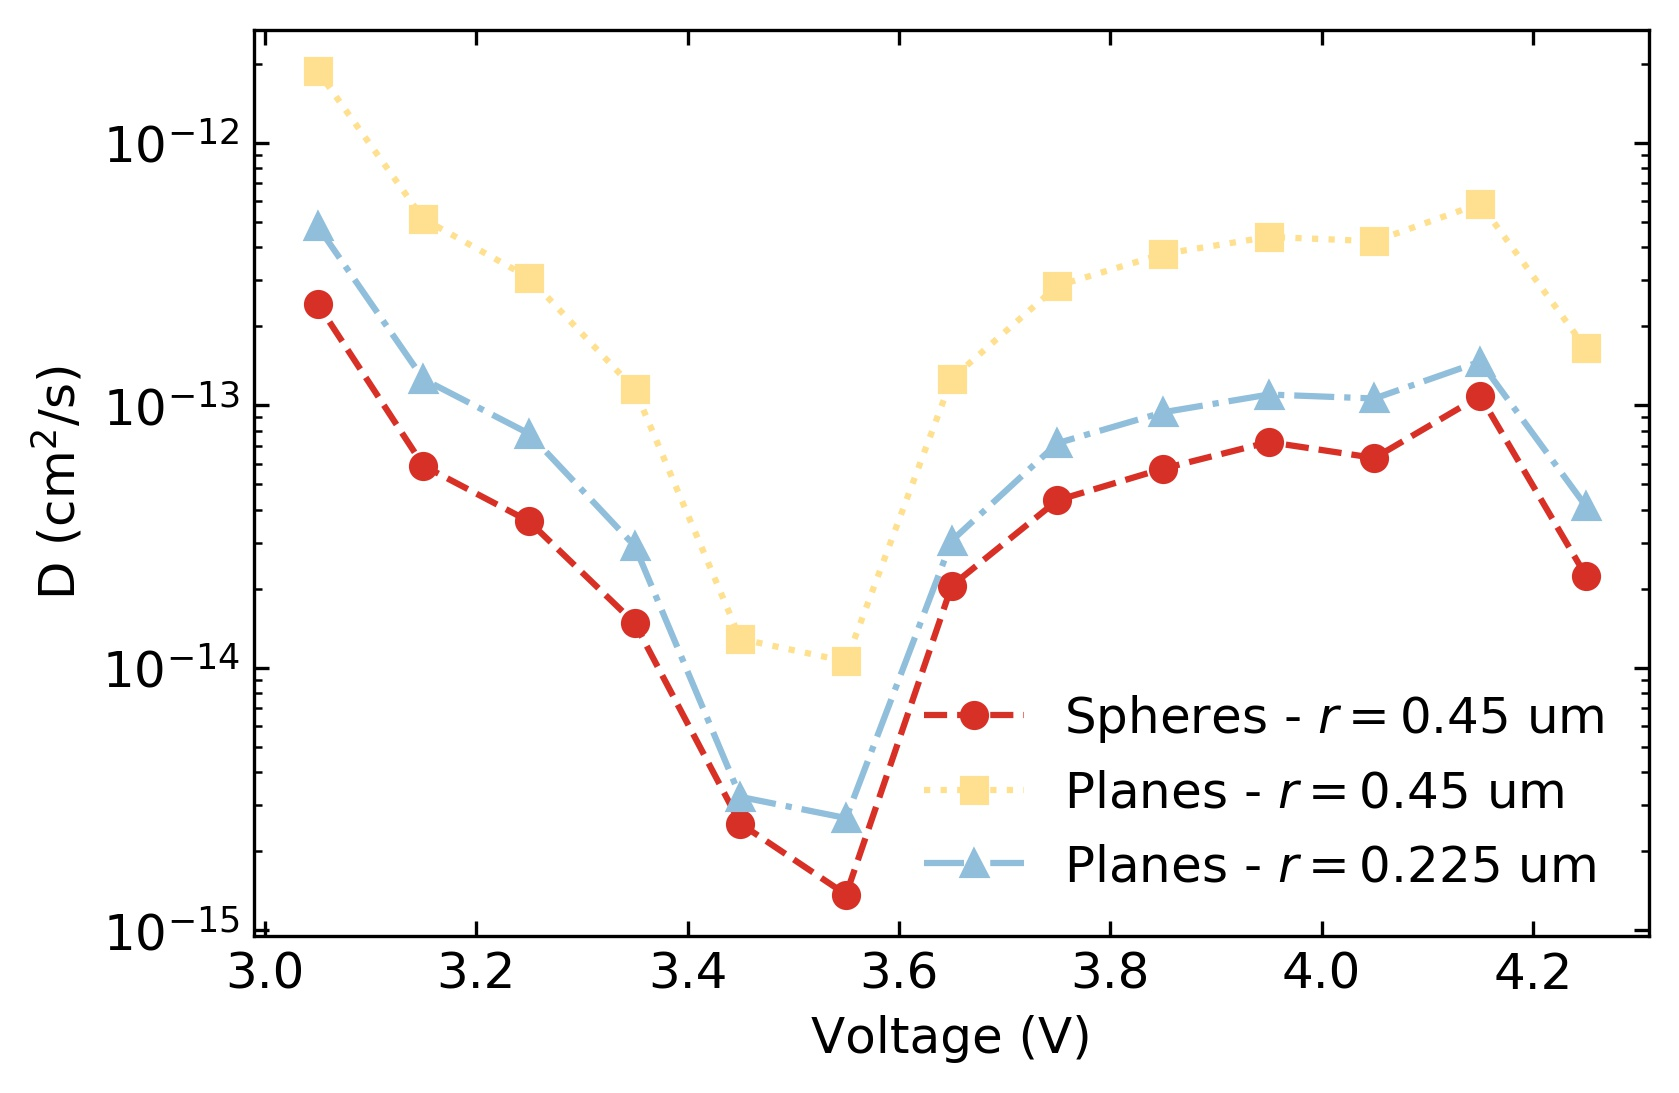
\includegraphics[width=0.75\linewidth]{figs/SC_Ni975Mg025_09um_30C_D-V_compare_sphere-plane.jpg}
\end{figure}

\end{frame}

\begin{frame}
\frametitle{How to obtain D for full V range?}

\begin{figure}
	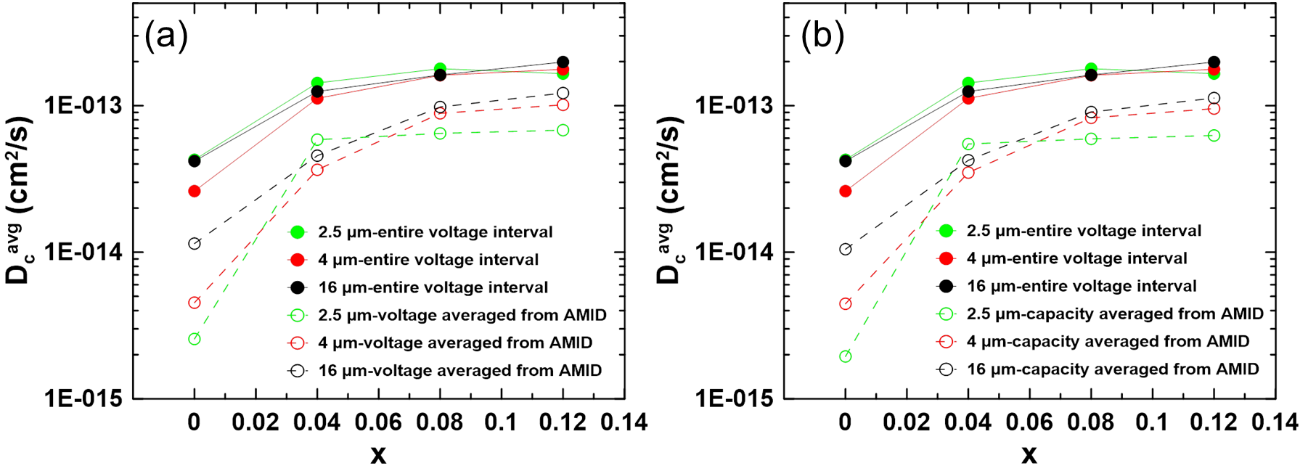
\includegraphics[width=0.95\linewidth]{figs/avgD.png}
\end{figure}

Recall: solution to couple PDEs assume D was constant. \\
Provided modest IR, I trust D(V) data more than full range D.

\end{frame}

\begin{frame}
\frametitle{AMID tells us the positive electrode rate capability}

\centering
Li$_{1+x}$(Ni$_{0.5}$Mn$_{0.5}$)$_{1-x}$O$_2$
\vspace{-0.5cm}
\begin{columns}
	
	\column{0.5\textwidth}
	\begin{figure}
		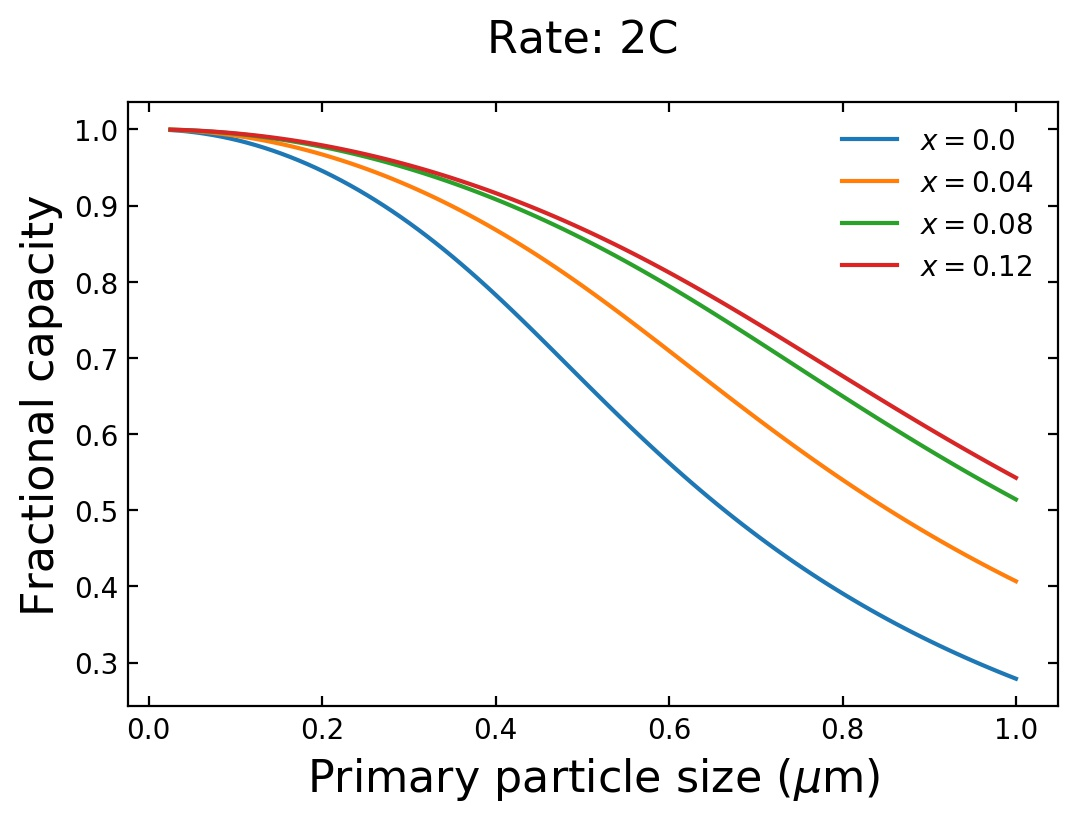
\includegraphics[width=0.95\linewidth]{figs/cap-primsize_2C.jpg}
	\end{figure}
	
	\column{0.5\textwidth}
	\begin{figure}
		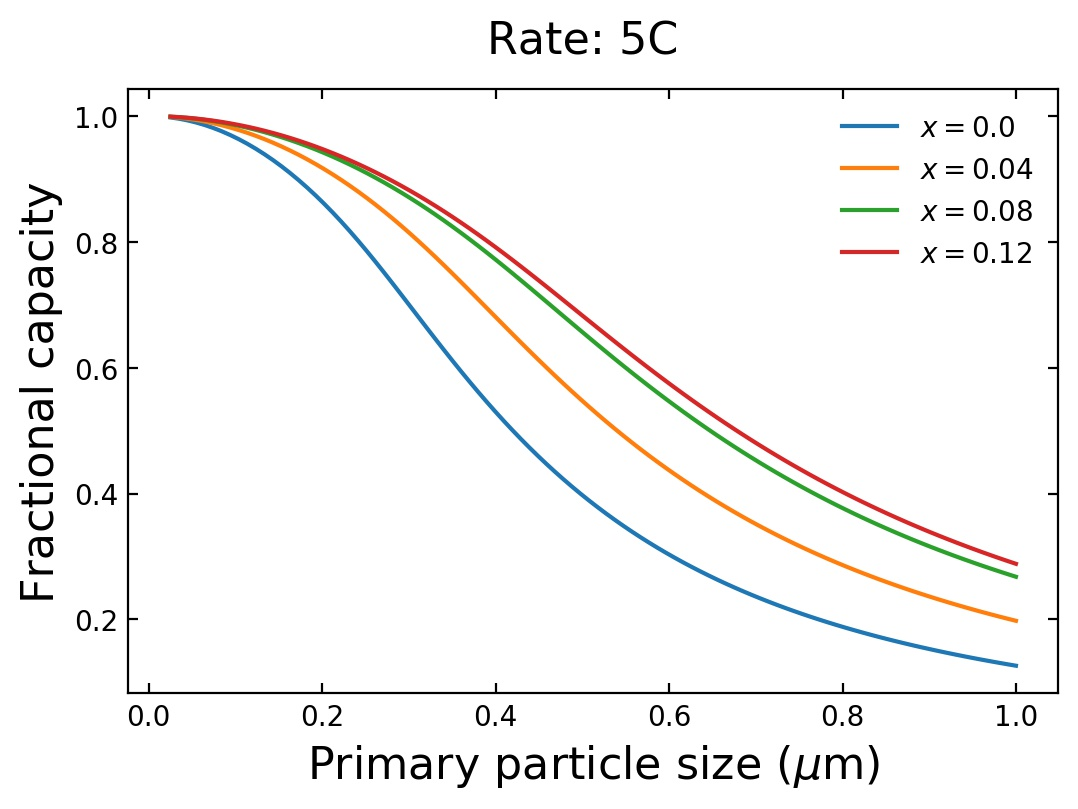
\includegraphics[width=0.95\linewidth]{figs/cap-primsize_5C.jpg}
	\end{figure}
	
\end{columns}

Assuming no other kinetic limitations in the cell (i.e., electrolyte)

\end{frame}

\begin{frame}
\frametitle{Can we correct for IR?}

\begin{figure}
	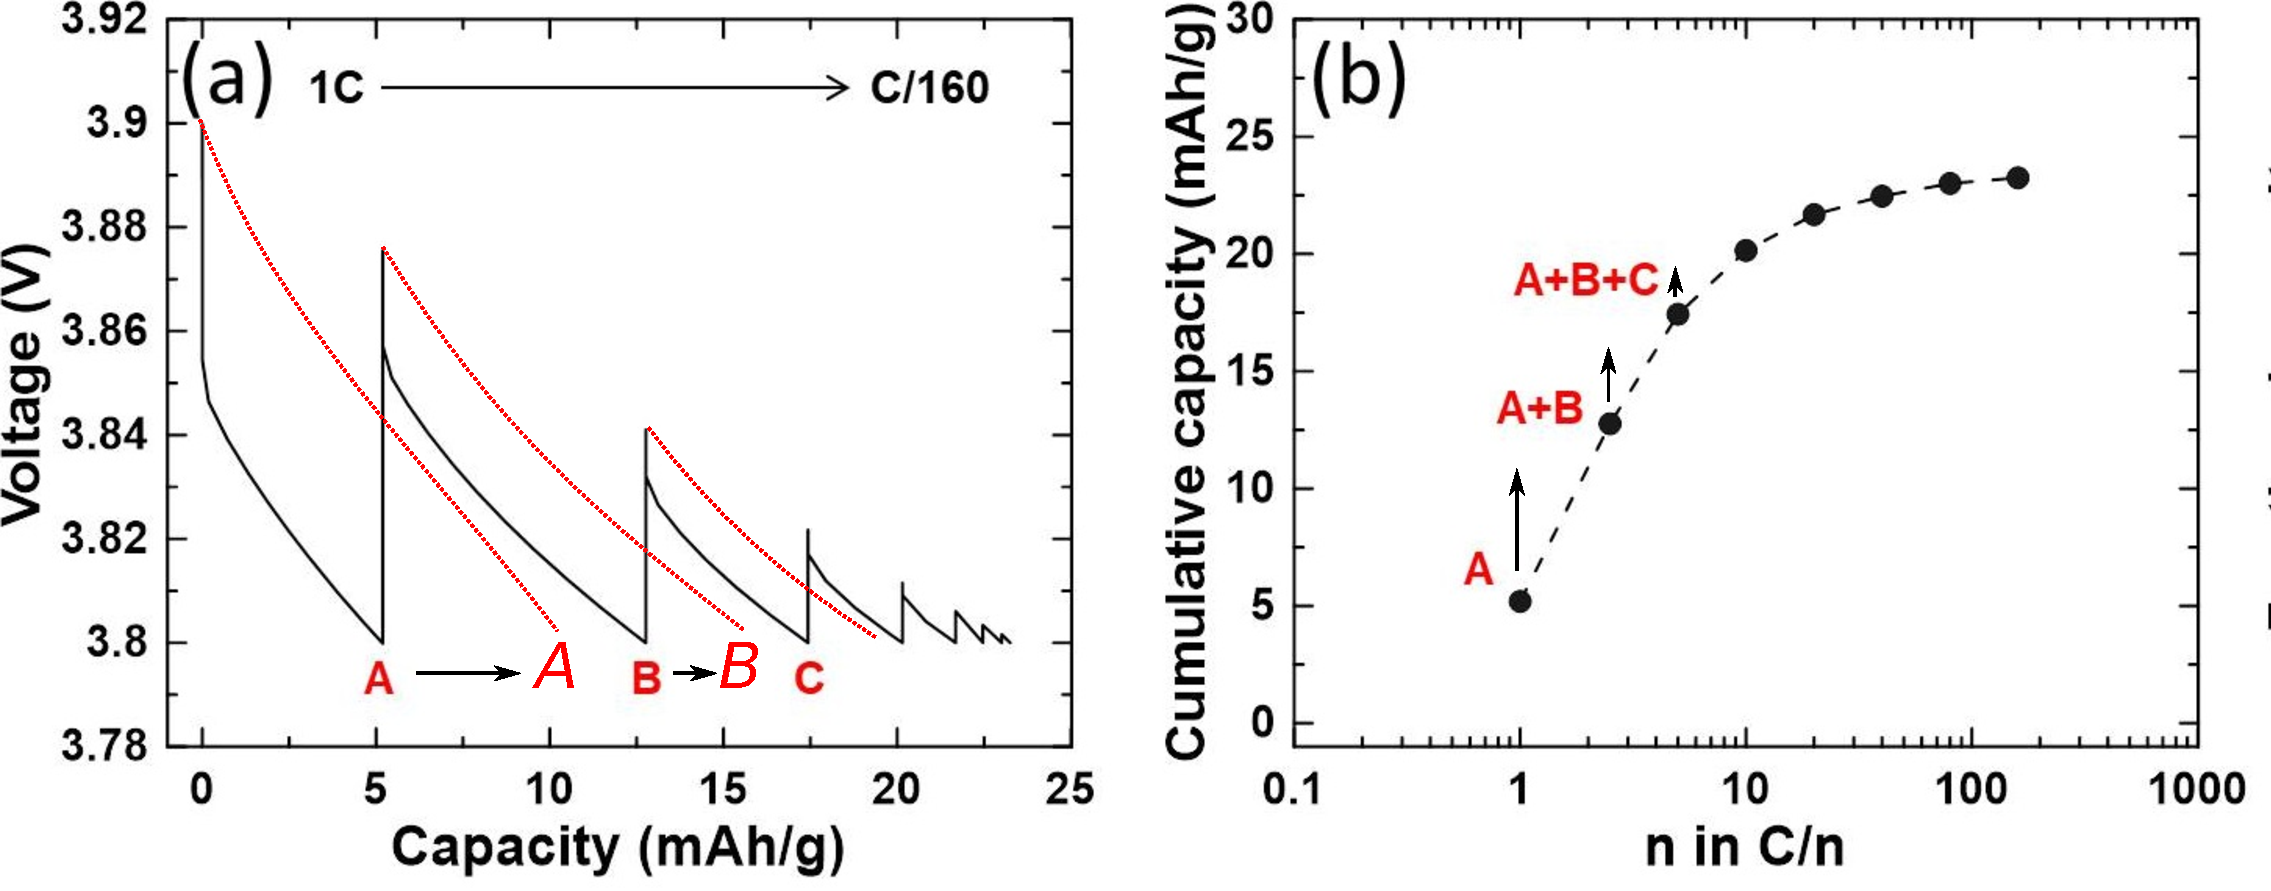
\includegraphics[width=0.95\linewidth]{figs/IR_correct.pdf}
\end{figure}

\end{frame}

\begin{frame}
\frametitle{Install AMID API and Jupyter Notebook}
\fontsize{10}{10}
\begin{itemize}
	\item Install Python through Anaconda: https://www.anaconda.com/products/individual
	\item Install spyder-notebook. In Windows search bar type ``Conda prompt". Then run ``conda install spyder-notebook".
	\item Create folder ".matplotlib\textbackslash stylelib" (if it does not exist already) in your home directory.\\
		  On Windows: ``C:\textbackslash \textbackslash Users\textbackslash user\_name\textbackslash"
	\item Copy grapher.mplstyle from ``dahn-share\textbackslash marc~cormier\textbackslash amid-api\textbackslash" into the 
	      ``.matplotlib\textbackslash stylelib\textbackslash" folder.
	\item Copy ``amid.py" and ``amid-analysis.ipynb" into the same folder, wherever you like on your computer.
	\item Open Spyder. If you don't see a ``Notebook" tab, select View$\rightarrow$panes$\rightarrow$Notebook.
	\item Use the small gear wheel in the top right of the Notebook panel to open amid-analysis.ipynb
\end{itemize}

\end{frame}


\end{document}